\documentclass[11pt,oneside]{article}
\input{coursHeadings}

\usepackage[%
    pdftitle={TD Communication technique},
    pdfauthor={Xavier Pessoles},
    colorlinks=true,
    linkcolor=blue,
    citecolor=magenta]{hyperref}



% \makeatletter \let\ps@plain\ps@empty \makeatother
%% DEBUT DU DOCUMENT
%% =================
\sloppy
\hyphenpenalty 10000

\newcommand{\Pointilles}[1][3]{%
\multido{}{#1}{\makebox[\linewidth]{\dotfill}\\[\parskip]
}}


\begin{document}


\newboolean{prof}
\setboolean{prof}{false}
%------------- En tetes et Pieds de Pages ------------
\pagestyle{fancy}
\renewcommand{\headrulewidth}{0pt}

\fancyhead{}
\fancyhead[L]{%
\begin{minipage}[c]{1.6cm}
\includegraphics[width=2cm]{png/logo_ptsi.png}%
\end{minipage}
\rule{2cm}{.5pt}
}

\fancyhead[C]{\rule{11cm}{.5pt}}

\fancyhead[R]{%
\begin{minipage}[c]{3cm}
\begin{flushright}
\footnotesize{\textit{\textsf{Sciences Industrielles\\ pour l'Ingénieur}}}%
\end{flushright}
\end{minipage}
}

\renewcommand{\footrulewidth}{0.2pt}

\fancyfoot[C]{\footnotesize{\bfseries \thepage}}
\fancyfoot[L]{\footnotesize{2011 -- 2012} \\ X. \textsc{Pessoles}}
\ifthenelse{\boolean{prof}}{%
\fancyfoot[R]{\footnotesize{TD -- CI 5 : Communication technique -- P}}
}{%
\fancyfoot[R]{\footnotesize{TD -- CI 5 : Communication technique}}
}


%\begin{center}
%\textit{Centre d'intérêt}
%\end{center}


\begin{center}
 \huge\textsc{CI 5 -- Communication technique}
\end{center}

\begin{center}
 \LARGE\textsc{Représentation des pièces mécaniques}
\end{center}

\vspace{.5cm}

\textit{D'après document de Jean-Pierre Pupier}

\begin{contexte}
\begin{itemize}
\item Contexte technique : représentation de pièces géométriques diverses
\item Objectif : savoir passer d'une représentation 3D à une représentation 2D en respectant les normes de représentation.
\end{itemize}
\end{contexte}

\section{Les projections de base}
\subsection{Pièces simples}
\begin{center}
\includegraphics[width=.9\textwidth]{png/fig1}
\end{center}

\begin{center}
\includegraphics[width=.9\textwidth]{png/fig2}
\end{center}

\begin{center}
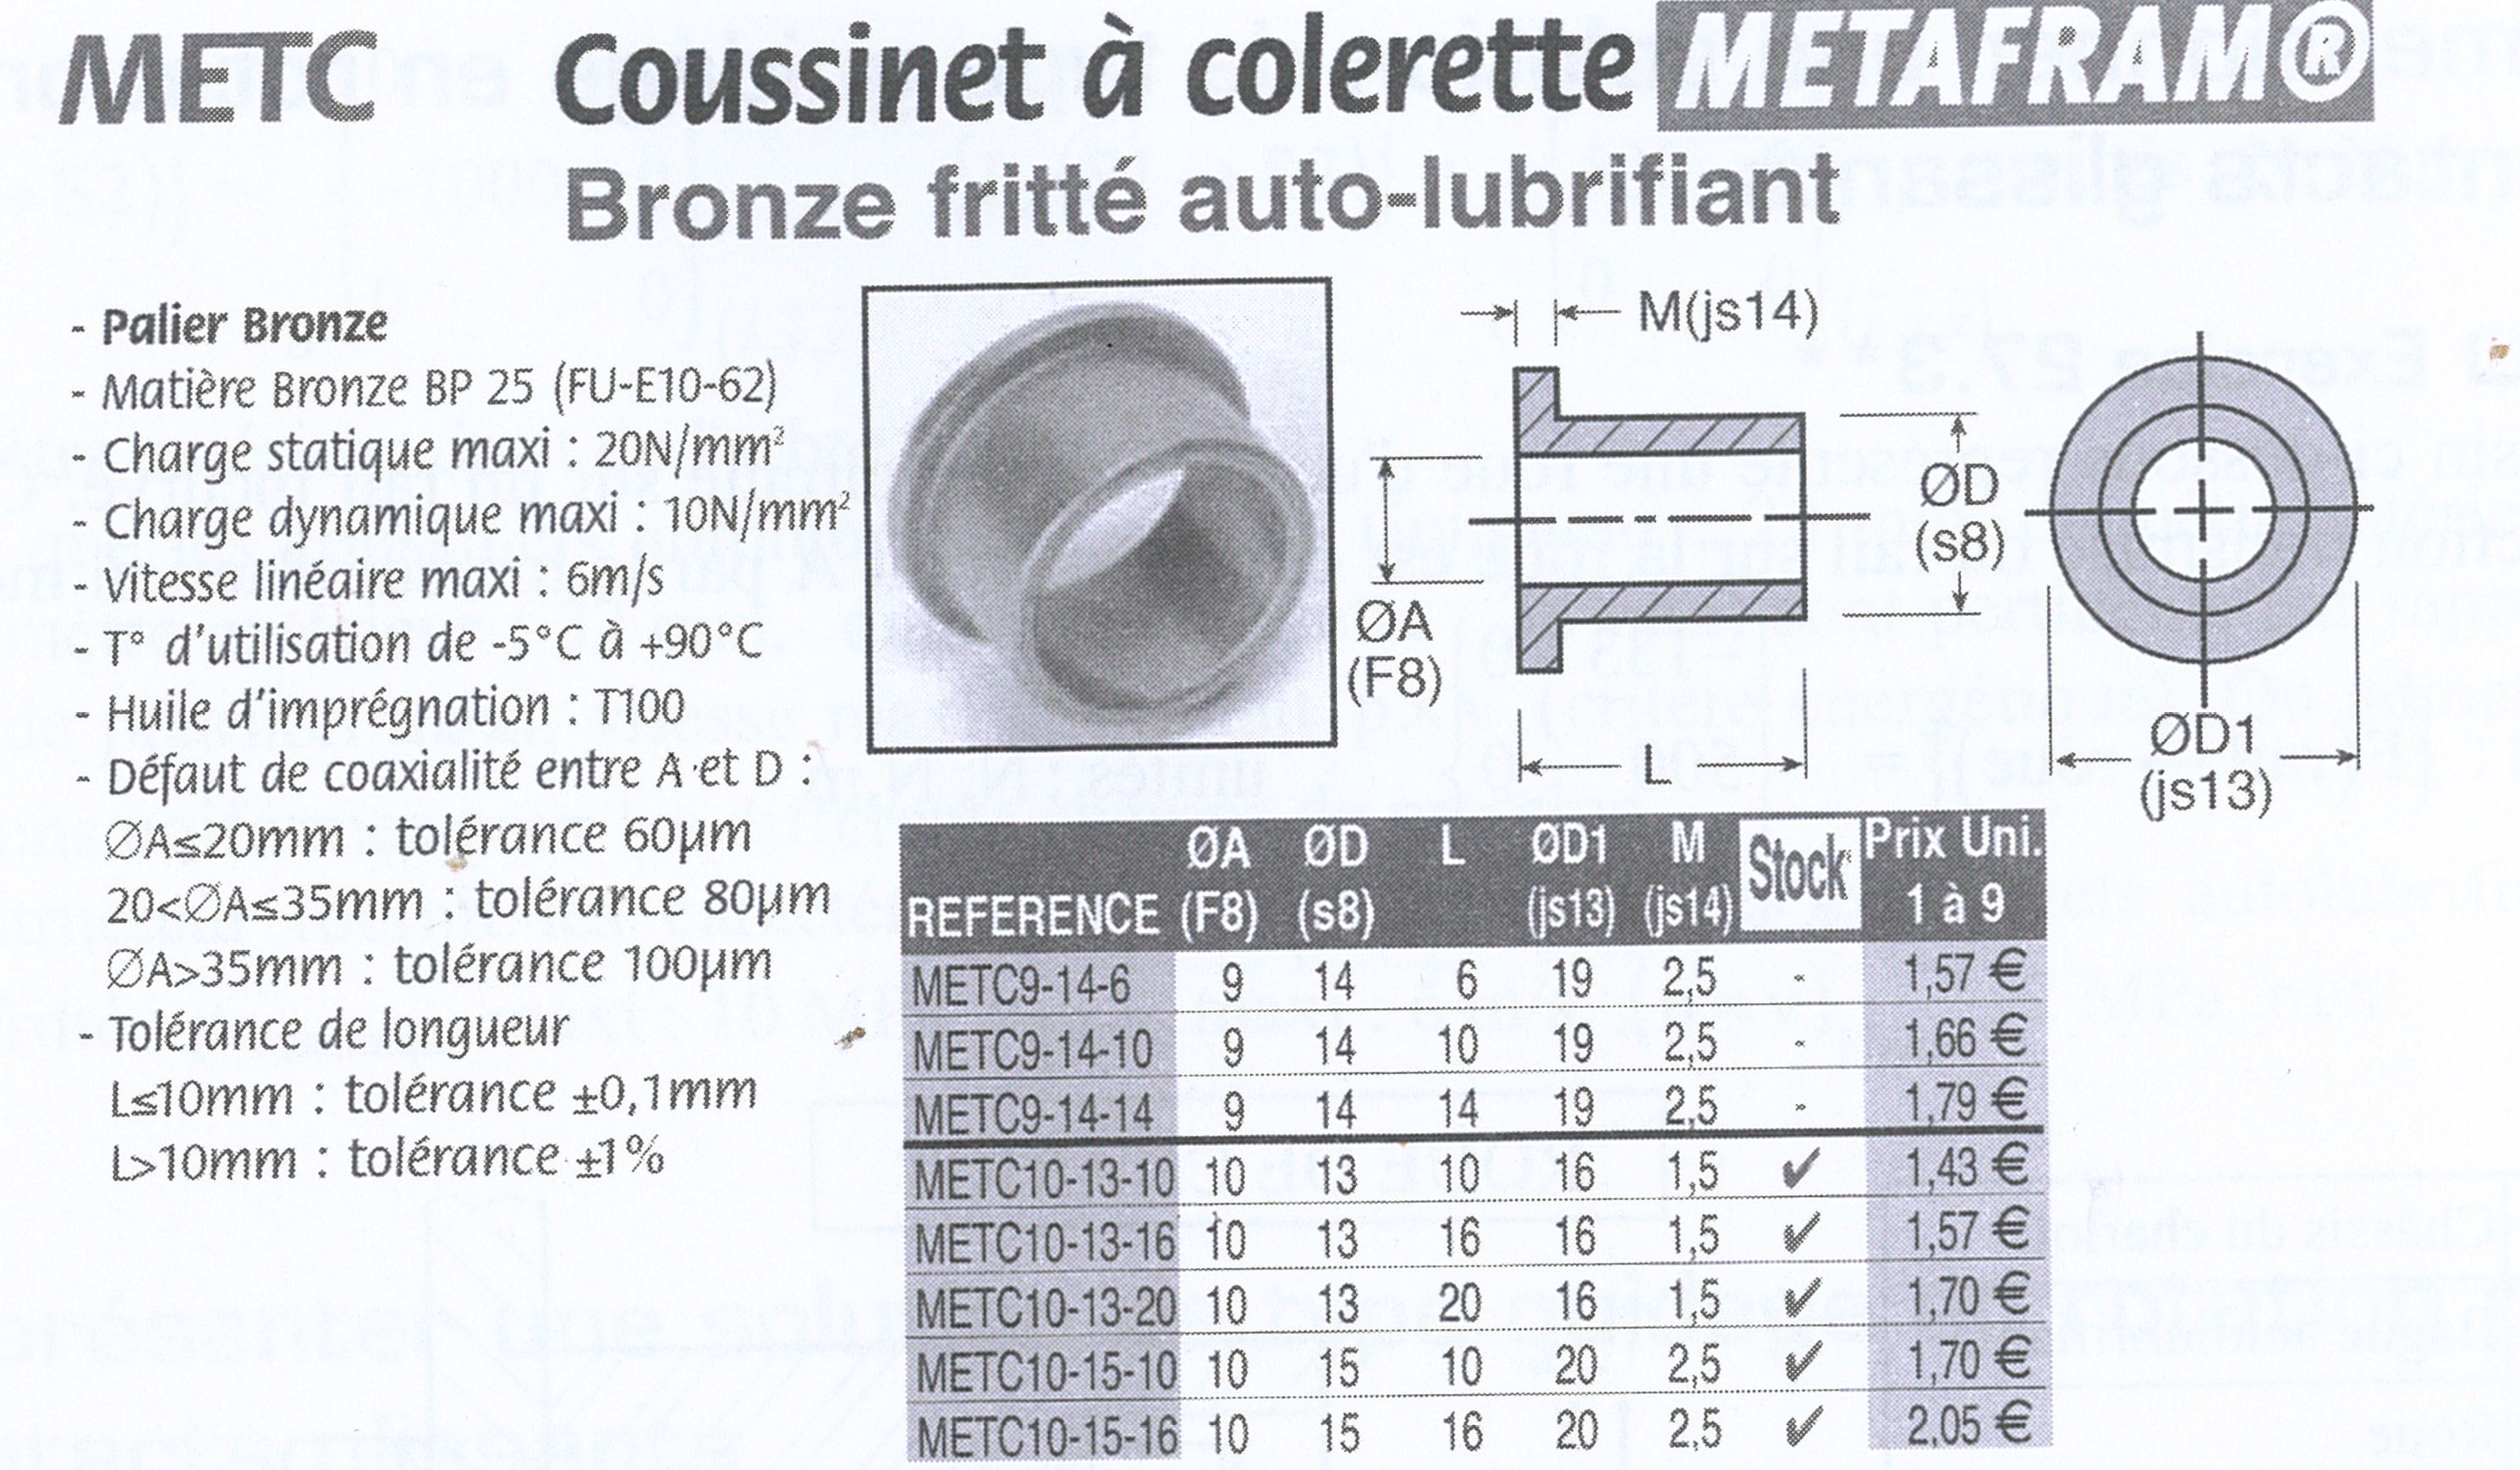
\includegraphics[width=.9\textwidth]{png/fig3}
\end{center}

\begin{center}
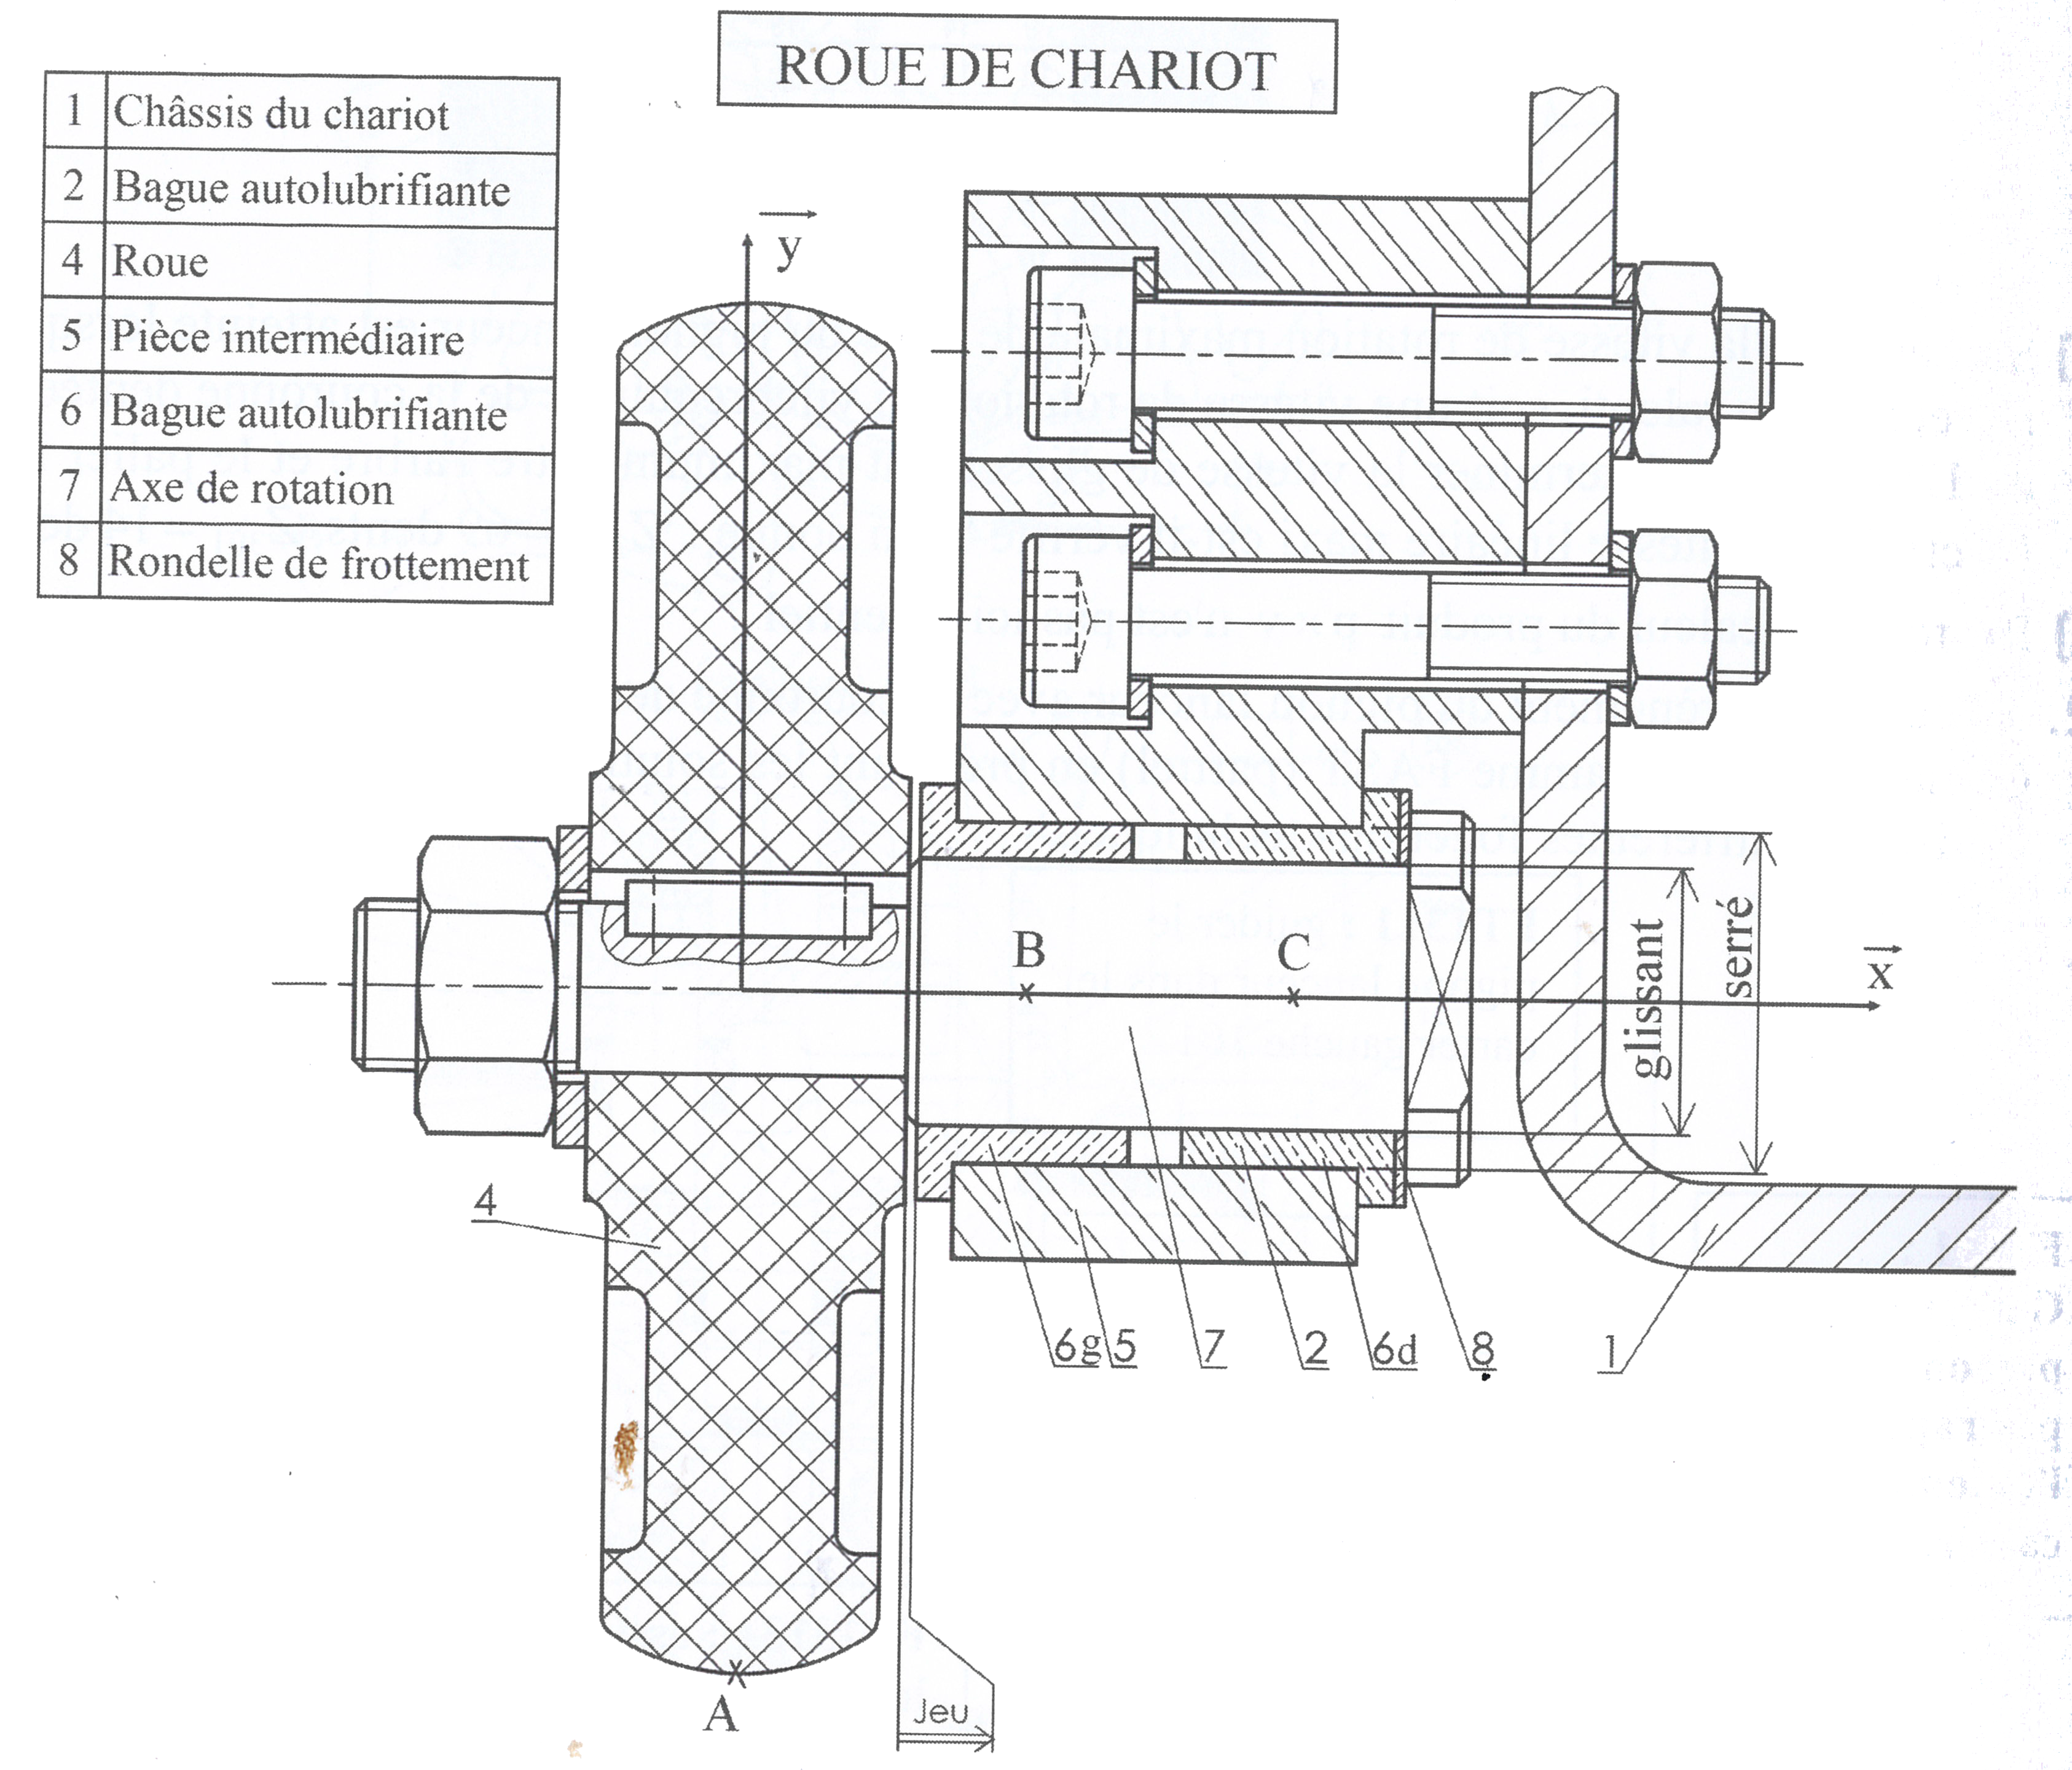
\includegraphics[width=.9\textwidth]{png/fig4}
\end{center}

\begin{center}
\includegraphics[width=.9\textwidth]{png/fig5}
\end{center}

\subsection{Pièces plus complexes}
\begin{center}
\includegraphics[width=.9\textwidth]{png/fig6}
\end{center}

\begin{center}
\includegraphics[width=.9\textwidth]{png/fig7}
\end{center}

\begin{center}
\includegraphics[width=.9\textwidth]{png/fig8}
\end{center}

\subsection{Vues de face, de dessus, etc...}

\subsubsection{Porte-outil complet en représentation perspective}
\begin{center}
\includegraphics[width=.9\textwidth]{png/fig9}
\end{center}

\subsubsection{Dessin de définition complet de la pièce 3 appelée porte-outil}

\begin{center}
\includegraphics[width=.9\textwidth]{png/fig10}
\end{center}


\subsubsection{Travail à réaliser : compléter le dessin de définition de la pièce 1
(corps)}

\begin{center}
\includegraphics[width=.9\textwidth]{png/fig11}
\end{center}

\begin{center}
\includegraphics[width=.9\textwidth]{png/fig12}
\end{center}

\section{Les coupes et les sections}
%\subsection{Les sections}
%\subsubsection{Sections sorties}
%\subsubsection{Sections rabattues}
%\subsection{Les coupes}
%\subsubsection{Coupe par une seul plan et demi-coupe}
%\subsubsection{Coupe brisée à plans parallèles ou à plans sécants}
%\subsubsection{Coupe des nervures et coupe locale}
%\subsubsection{Éléments non coupés}
\subsection*{Application - levier}
\subsubsection*{Perspective sommaire}

\begin{center}
\includegraphics[width=.6\textwidth]{png/fig13}
\end{center}

\subsubsection*{Dessin de définition à compléter}

\begin{center}
\includegraphics[width=.9\textwidth]{png/fig14}
\end{center}
%
%\begin{center}
%\includegraphics[width=.9\textwidth]{png/fig15}
%\end{center}
%
%\begin{center}
%\includegraphics[width=.9\textwidth]{png/fig16}
%\end{center}

\section{Intersection de cylindres}
\subsection{Cylindres pleins même diamètre}
\begin{center}
\includegraphics[width=.9\textwidth]{png/fig17}
\end{center}

\subsection{Cylindres pleins diamètres différents}
\begin{center}
\includegraphics[width=.9\textwidth]{png/fig18}
\end{center}

\subsection{Cylindres creux même diamètre}
\begin{center}
\includegraphics[width=.9\textwidth]{png/fig19}
\end{center}

\subsection{Cylindres creux diamètres différents}
\begin{center}
\includegraphics[width=.9\textwidth]{png/fig20}
\end{center}

\section{Autres exercices}

\begin{center}
\includegraphics[width=.9\textwidth]{png/fig21}
\end{center}

\begin{center}
\includegraphics[width=.9\textwidth]{png/fig22}
\end{center}

\begin{center}
\includegraphics[width=.9\textwidth]{png/fig23}
\end{center}


\end{document}